\begin{figure}[h]
    \centering
    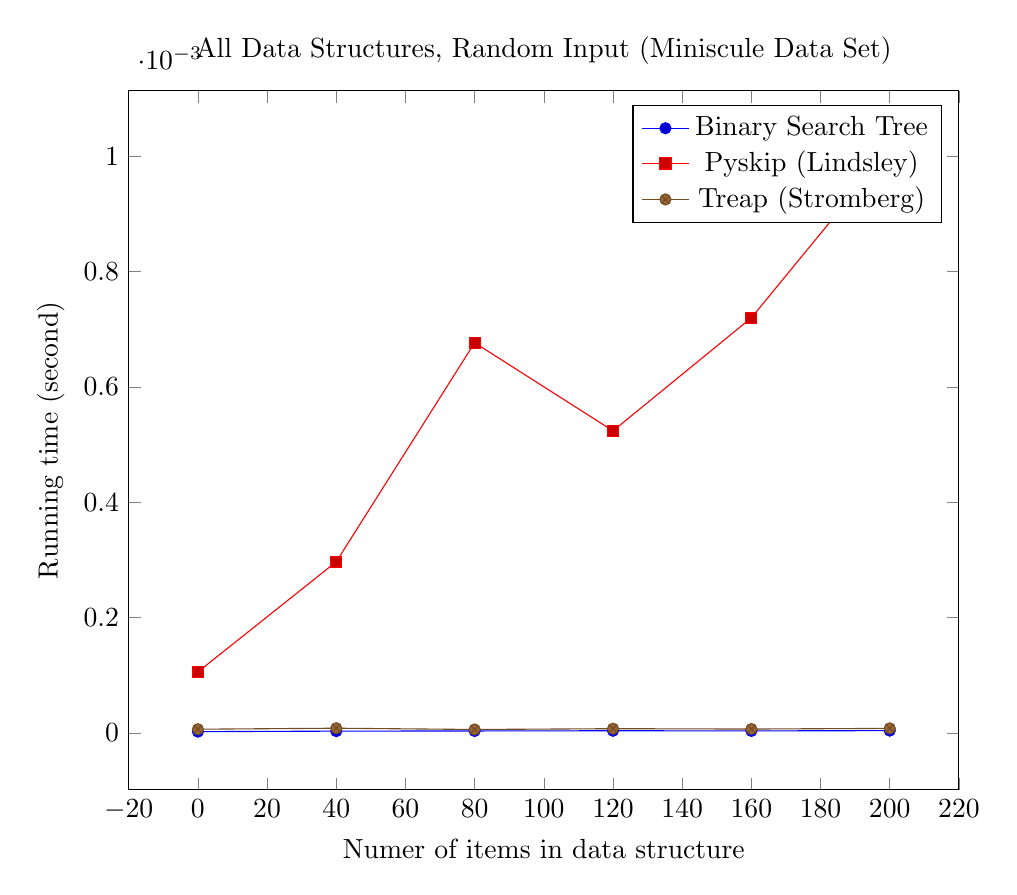
\begin{tikzpicture}
        \begin{axis}[
            xlabel={Numer of items in data structure},
            ylabel={Running time (second)},
            title={All Data Structures, Random Input (Miniscule Data Set)},
            width=\textwidth
        ]
		\addplot coordinates {
			(0, 2.1383448909368815e-06)
			(40, 3.041870901191902e-06)
			(80, 3.3430462379435777e-06)
			(120, 3.704456642045586e-06)
			(160, 3.4635163726442436e-06)
			(200, 3.9152793777717585e-06)
		};
		\addplot coordinates {
			(0, 0.0001057426607335125)
			(40, 0.0002967480593014238)
			(80, 0.0006765903940126342)
			(120, 0.0005237740281448355)
			(160, 0.0007197789373028244)
			(200, 0.0010121900717550245)
		};
		\addplot coordinates {
			(0, 6.3849171391350264e-06)
			(40, 8.101616558620073e-06)
			(80, 5.903036600332645e-06)
			(120, 7.258325615713823e-06)
			(160, 6.686092475885475e-06)
			(200, 7.80044122186685e-06)
		};
        \legend{Binary Search Tree, Pyskip (Lindsley), Treap (Stromberg)}
        \end{axis}
    \end{tikzpicture}
    \caption{Average of 10 operations, benchmarked every 40, starting at 0.}
\end{figure}